\documentclass[conference]{IEEEtran}

\ifCLASSINFOpdf
 \usepackage[pdftex]{graphicx}
\else
\fi
\bibliographystyle{plain}



\begin{document}
\title{XCPU3: Workload distribution and aggregation}


\author{\IEEEauthorblockN{Pravin Shinde}
\IEEEauthorblockA{Parallel and Distributed Systems(PDCS)\\
Vrije Universiteit, Amsterdam\\
Email: pse220@few.vu.nl}
\and
\IEEEauthorblockN{Eric Van hensbergen}
\IEEEauthorblockA{IBM Research Lab\\
Austin, USA\\
Email: ericvanhensbergen@us.ibm.com}}

\maketitle

\begin{abstract}


As clusters and grids are reaching to domains like commercial application, it
is becoming more clear that the existing workload distribution solutions which
are tailored for high performance scientific applications, are not efficient
for dynamic data-flow applications and many-task computing (MTC).

Most of the existing workload distribution solutions that concentrate more on
HPC applications and are not efficient in quickly deploying the dynamic
workload involving large number of small jobs which is the typical case in
dataflow applications. Also developing and deploying applications on existing
infrastructures still is a non-trivial task requiring special runtimes,
middleware support and/or language dependence.

We have explored an alternate approach for simplifying workload
distribution and aggregation based on synthetic filesystems and the private
namespace concepts of Plan 9.  Instead of sending workloads to a remote
cluster, XCPU3 works by bringing the remote cluster to the user's desktop,
leading to full control over the compute environment.   XCPU3 provides
a filesystem interface, making it runtime and language agnostic.  It also
allows executing multiple jobs simultaneously in isolation, leading to
better resource utilization.  XCPU3 makes all nodes independent and
equivalent in functionality leading to the ability to localize the
decision making and ability to handle dynamic workloads.  XCPU3 provides easy to
use, flexible and scalable infrastructure for workload distribution and
aggregation that can be used by dynamic workloads and dataflow applications.

\end{abstract}

\IEEEpeerreviewmaketitle

\section{Introduction}

Due to the limits on the silicon technology, the trend is moving in the
direction of multicore and manycore architectures.  Having a large number of
less powerful computers is assumed to be economically more viable than having a
single more powerful computer.  The increasing acceptance of clusters and
grids coupled with the emergence of cloud computing and availability of compute
resources as utility via \cite{ec2} \cite{azure} \cite{appengine} has increased
the need for parallel programming and workflow management.

The initial development around parallel programming and the traditional
infrastructure around clusters and grids is designed to suit the
requirements of the scientific community which tend to run large compute
intensive applications for long durations.  With growing use of clusters and
grid, there is increasing interest in deploying new genre of applications like
dataflow applications and many-task applications. Typical commercial
applications fall into the category of dataflow applications and involve
executing lot of small and interdependent applications for small amount of time.
Unfortunately, most of the existing workload deployment solutions are ill-suited
for these applications. These solutions are efficient in deploying large
compute-intensive application which will run for long duration, but are highly
inefficient in deploying large number of small applications for small amount of
time.

The major obstacle in widespread adoption is the expertise needed for writing
parallel applications.  Also, dependence on a specific language or runtime
environment for parallelism dictates the need for major re-writing all existing
applications for exploiting the parallelism.


Another crucial property exhibited by dataflow applications is that the amount
of resources needed for total computation is unpredictable in the beginning as
it may depend on results of intermediate computations.  This leads to the
requirement of dynamically allocating new resources whenever needed. Most of the
current job schedulers do not support such adaptability and flexibility.


In this paper, we target the problem of creating a scalable infrastructure
with the flexibility needed for running dataflow applications.  We primarily
target the Blue Gene \cite{bgp} supercomputer as our testbed as it allows us to
test our infrastructure on up to 64K nodes.


The challenge is to provide the flexibility needed by dataflow applications
using a very simple interface.  We need to provide an infrastructure with
support for dynamically adjusting the resource reservation which can help in
coping with unpredictable resource requirements.  This infrastructure needs to
provide quick job-startup time even for large numbers of jobs, allowing overall
good performance for dataflow applications.  It also needs to provide a simple
interface for communication between nodes even when those nodes cannot
communicate directly with each other. We do not want the application development
for this infrastructure to be constrained to a particular language, runtime,
middle-ware or platform.  And we need to run most of the existing applications
without modification.


Our primary aim is not performance improvement, but to present a new and elegant
way for workload distribution and aggregation.  It is aimed at demonstrating
that simple filesystem interfaces and a simple design based on the basic
principles of the Plan 9 \cite{pike95plan} distributed operating system can be
easy, intuitive and scalable to a large number of nodes.

This paper is organized as follow. The next section presents the background
work which has inspired this project. The \textit{Design section} will discuss
the design and the reasoning behind it. \textit{Implementation section} will
discuss how system is implemented. The \textit{Filesystem interface section}
explains the use of synthetic filesystem and presents few examples to show how
easily this interface can be used. Evaluations section presents some results
showing that this approach is feasible. Related work section positions XCPU3 in
the context of other related projects. Conclusion section will conclude this
project.

%%%%%%%%%%%%%%%%%%%%%%%%%%%% End of Introduction chapter %%%%%%%%%%%%%%%%%%%%%%%

%%%%%%%%%%%%%%%%%%%%%%%%%%%% Start of Background chapter %%%%%%%%%%%%%%%%%%%%%%%

\section{Background}
This section discusses the the previous work from which XCPU3 is evolved.

\subsection{Plan 9}
Plan 9 is an operating system which was specifically designed for dealing with
networked systems.  It is based on principles like \textit{everything is file}
and \textit{private namespaces}\cite{namespace}.  It provide applications
ability to build custom namespace by mounting and binding remote resources and
then run in network oblivious manner.  The usefulness of these features can be
seen in CPU\cite{plan9-cpu} which is Plan 9's way for using remote compute
resources.  Unlike Unix based remote login and SSH where remote processes run
in the namespace and environment of remote node, CPU runs the remote processes
in local namespace and environment.  One of the key advantages of this model
simplifies the remote workload deployment as even though workload runs on
remote resources, it runs in local environment without getting affected by the
environment on remote node.

\subsection{XCPU}
XCPU\cite{ron-xcpu} \cite{lucho-xcpu} was an attempt to bring the functionality
of CPU into mainstream operating systems like Linux.  XCPU allows process
management using a \textbf{filesystem interface}.  As this underlying psudo
filesystem can be exported over network to other nodes, it simplifies the
sharing of the compute resources.  XCPU does not provide private namespace,
which is needed for transparantly accessing remote filesystem.  XCPU works
around this limitation by pushing the executables and it's dependencies needed
for requested remote execution.

To achieve scalable pushing of programs and their dependencies, XCPU uses a few
compute nodes for distributing the programs and dependencies during the program
startup time creating a tree hierarchy of the nodes.  This is known as the
\textbf{tree spawn mechanism} and it improves the scalability for XCPU to
larger numbers of nodes. With automatic pushing and the tree spawn mechanism,
XCPU not only simplifies the deployment of applications but it also scales
them better with quicker job startup time.

\subsection{XCPU2}
XCPU2 \cite{lucho-xcpu2} is evolved from XCPU and is aimed to give more
flexibility by using \textit{private namespace} support added recently into
Linux kernel\cite{linuxns}.  This allows remote processes to execute in the
namespace which provides local filesystem view.  By controlling the
environment and filesystem view of all the remote processes, every developer
is free to use any libraries and development setup, regardless of what is
installed on remote nodes.  As these processes run in the isolation provided by
the private namespace, they do not pollute the environment and filesystem view
of other processes.  This allows executing multiple processes of different
users on same remote node without conflicting with each other.

XCPU2 makes clear distinction between various nodes which are assigned with
specific responsibility.  The nodes are classified into \textit{control node}
which is responsible for reserving the compute nodes, \textit{job control node}
which are responsible remote job management and namespace management on compute
nodes. The \textit{compute nodes} are responsible for actual computation
by running the processes on inside custom namespace on users behalf.
 
The XCPU2 lacks fine-grained granularity of the control.  It only supports
managing all \textit{compute nodes} together in identical way, and does not
give any mechanism to control each \textit{compute node} individually.  This
lack of control on every node is a major deterrent for dataflow applications.
This limitation was major motivation for us to develop XCPU3 for providing much
needed flexibility and fine grained control over over all compute nodes using
simple interface.


%%%%%%%%%%%%%%%%%%%%%%%%%%%% End of Introduction chapter %%%%%%%%%%%%%%%%%%%%%%%
%%%%%%%%%%%%%%%%%%%%%%%%%%%% Start of Design chapter %%%%%%%%%%%%%%%%%%%%%%%

\section{Design}

The key challenge in this design was to provide the flexibility needed by
dataflow applications while achieving scalability to the large number of nodes
available. 

\subsection{Key design decisions}

We decided to adopt a few guiding principles which will help us to reach our
goal of flexibility with scalability.  We also decided to keep the design simple,
and we believe that the simple design should lead to the simple and flexible
interface. We also hope that the lack of complexity may help in improving
scalability. In this section we present those decisions which influenced most
aspects of system design and implementation.

\subsubsection{Localization of decision making}
The key requirement for us was scalability to a large number of nodes.  We
planned to design the system without any central component which should have
knowledge of the entire system.  We plan to distribute and localize the
computations as well as decisions like scheduling, job management and
workload distribution/aggregation.

We avoid decision making based on global knowledge and promote use of local
information.  We hope that if each node tries to attempt a local optimum, we
will reach the global optimum.  This may not be true in all cases, We hope
that in those cases, we hope to perform acceptably well if not optimal.


\subsubsection{Independence of every node}
As we plan to distribute and localize all functionalities, it was essential to
replicate these functionalities at multiple levels making localization
possible.  The granularity of functionality replication decides the granularity of control,
and hence influences the flexibility provided by the system.  As we aim for 
maximum flexibility, we have decided for replicating the following three
functionalities at each node.
\begin{enumerate}
\item \textbf{Resource reservation}: Each node should be able to reserve more
resources on it's own without involvement of any central entity.

\item \textbf{Job management}: Every node should be capable of starting and
managing new jobs using his reservations.

\item \textbf{Computation}: Every node should be able to perform the
computation by running the requested application in isolation and returning
the results.
\end{enumerate}

We intend to provide each node with the capability to perform all of these roles
simultaneously instead of binding them in one role at one time.  This design
makes the interface to every node a building block identical to each other, 
and provides the flexibility to build any structure with these building blocks.

There are a few downsides in making every node independent.  With independence
of every node, each node can be a source of failures and faults.
One will need to come up with better ways to deal with faults and
failures when so many sources of them are present.  This takes the XCPU3 in
realms of \textbf{Distributed Systems} opening many more possibilities and
questions.

For purpose of this exploration, we avoid these complexities by assuming a very
simple model for handling failures.  Any failure anywhere in the system will
result in the failure of the entire operation.  We assume that failures will
be in-frequent, so aborting and restarting operation should be acceptable for
such infrequent failures.

\subsubsection{Filesystem Interface}
We want to keep XCPU3 interface agnostic from language, runtime and middleware.
Plan 9 has proven that the filesystem interface is very flexible and yet
powerful in the world of distributed applications.  We aim to follow the same
principle of \textbf{Everything is a file} from Plan 9.

Every node will provide access to its services via filesystem interfaces.
This interface will be exported as the filesystem over the network so that other
nodes can use it. Other nodes can mount this filesystem and use it as
interface for interacting with that node.  Multiple remote nodes can be
aggregated into the filesystem hierarchy providing a clean and easy way to
access them.

Multiple overlay views can be created by \textit{binding} the same filesystem
at multiple locations with different names.  This ability of creating ad-hoc
overlays allow users to arrange remote resources as per his needs without
worrying about their actual locations.

Other advantages of using filesystem interfaces are that 
\begin{enumerate}
\item Existing tools/commands used with traditional filesystem can be directly
used with XCPU3.

\item filesystems come with their own mechanism for access control list for
providing the security.  We can leave the security to these already proven 
mechanisms instead of implementing our own.

\item We inherit the ability to export, mount and bind the filesystem
without writing any explicit code for it.

\item Filesystem interfaces are simpler to program than socket interfaces.  This
can lead to simpler code and hence lesser bugs.

\item Users don't need special privileges or administrative access to interact
with the filesystem.  This simplifies the user experience in running XCPU3 based
applications.
\end{enumerate}

The filesystem interface has following limitations which affect our system
design.

\begin{enumerate}

\item The critical limitation concerns the POSIX standard for failure
reporting in filesystem.  POSIX standard dictates that file operations should
report their success or failure in the form of a single number which may not be
enough to provide the information about the reason behind failures.  Plan 9
overcomes this limitation by returning a string which can provide more
verbose information instead of a single number.  But this breaks the POSIX
compatibility.  So, we need to find an alternate way to report information
about failures in POSIX compatible way.

\item Another drawback is the way a failure of remote services is detected.
The filesystem interface relies on the underlying networking protocol for
detecting failures by waiting for timeouts, and then reporting them back to
users as an error.  This makes the filesystem interface less desirable where
quick failure detection and recovery is needed.


\end{enumerate}

Our decision to choose the filesystem interface despite of it's drawbacks is the
trade-off we are willing to do for flexibility and simplicity.  We limit
ourself with the assumption that failures will be infrequent.  With this
assumption, we are willing to accept the delays in reporting failures at the
remote end.


\section{Implementation}

This section discusses the implementation issues in more detail.  This chapter
concentrates on how XCPU3 was implemented and discusses implementation
decisions which have proven to be important.


\subsection{Inferno}
Inferno\cite{inferno} is an open source distributed operating system which is a 
direct descendant of the \textbf{Plan 9} operating system.  It runs natively on
multiple hardware platforms and can also run as a user-space application on
top of other operating systems.  For the purpose of this document
\textit{"hosted Inferno OS"} or \textit{"userspace Inferno"} refers to Inferno
running as user-space application on top of other operating systems.

As we are aiming for a flexible heterogeneous environment with different
operating systems and different architectures, we found the Inferno operating
system to be an attractive platform.  It allowed us to develop XCPU3 once and
easily deploy it on different platforms while enjoying the Plan 9 features
on all those platforms.

This decision does come with the cost of performance loss.  Each node needs
to run hosted Inferno in user-space which takes up some resources of the node. 
Our choice of Inferno gave us the flexibility and features of the Plan 9
operating system on other operating systems.  It allowed us to quickly
implement and deploy our filesystem on multiple platforms easily at the cost
of some performance.

\subsection{Implementation details}

XCPU3 is implemented as the filesystem in the Inferno kernel.  Figure 
\ref{fig:XCPU3} shows the placement of XCPU3 in the context of applications,
host operating system and the Inferno.

\begin{figure}[h]
  \begin{center}
    \leavevmode
      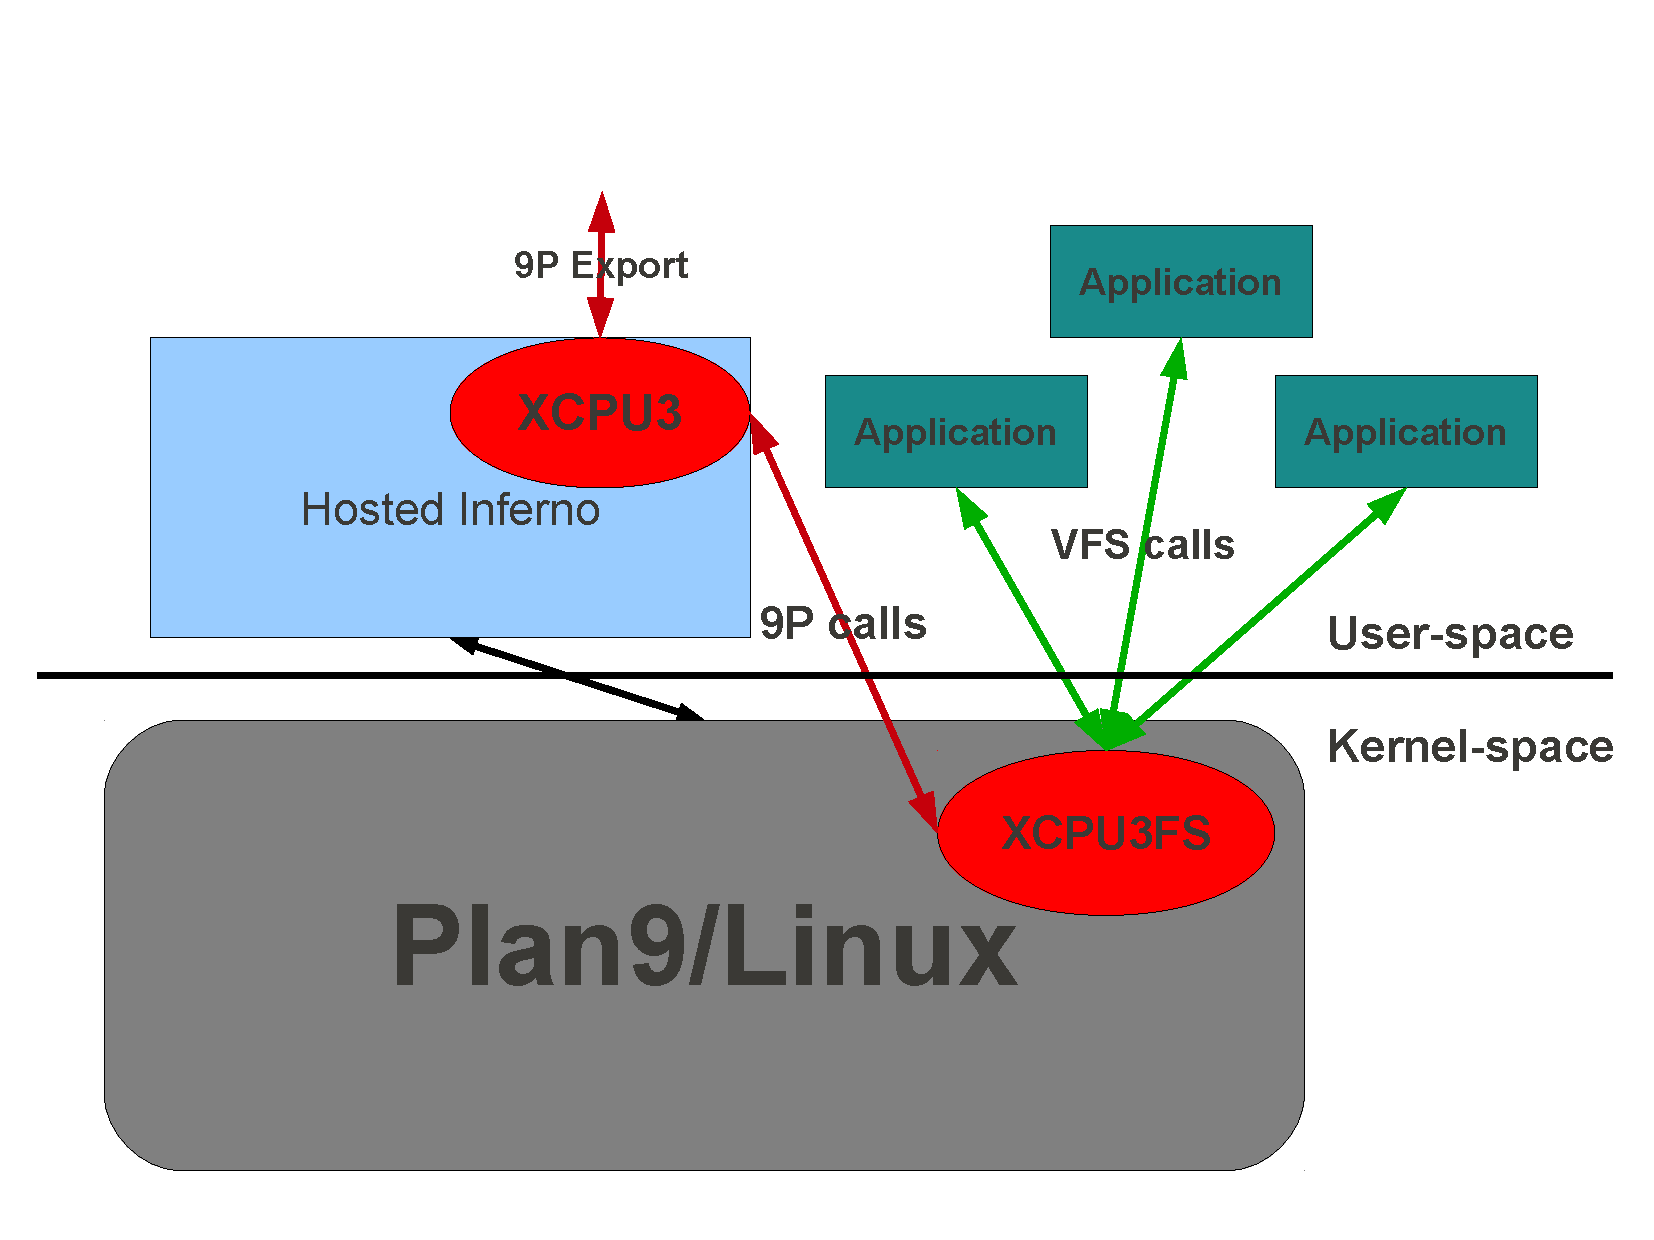
\includegraphics[height=0.2\textheight,width=0.5\textwidth]
		{./img/XCPU3Structure}
    \caption{XCPU3 Structure}
    \label{fig:XCPU3}
  \end{center}
\end{figure}

The XCPU3 filesystem is exported by Inferno using the \texttt{9P} protocol. 
This protocol is used by Plan 9 and Inferno extensively to access any file. 
Recently the Linux kernel has added support for the \texttt{9P}
protocol\cite{graverobbers}.  This allows Linux to mount filesystems
exported over the 9P protocol.  Other Unix based operating systems can use
FUSE\cite{FUSE} for accessing the 9P based filesystems. 

In a typical setup, Inferno runs in the hosted environment on an operating
system like Linux or Plan 9.  The hosted inferno will export the XCPU3
filesystem which can be mounted by the local host operating system. The 
applications interact with this mounted XCPU3 filesystem using the native
filesytem interfaces (e.g. VFS for Linux). Any interaction with this XCPU3
filesystem is communicated to Inferno using \textit{9P}. The XCPU3 kernel module
inside the inferno kernel then receives and interprets the user actions.  If
needed, it uses services from the host operating system or from other XCPU3
filesystems deployed on remote locations.  The XCPU3 filesystem then sends the
prepared response over 9P. The host operating system will relay this response
back to the application via the local filesystem interface.


\subsection{The big picture (connecting multiple XCPU3 nodes)}
The real power of the XCPU3 is the ability to connect with each other and form
bigger instance of XCPU3.  XCPU3 filesystem is exported over \texttt{9P}
providing same functionality and interface to both local and remote
applications.  This allows XCPU3 instances to connect with other XCPU3
instances and distribute some of their responsibilities among them.
The \texttt{9P} protocol shields the XCPU3 from complications of remote
filesystem access and works as transparant glue for connecting multiple XCPU3
instances together.

\subsubsection{Central Services}

The ability to configure many XCPU3 nodes into hierarchy is provided by the
\textit{central services}.  In contrary to the name, central services is
highly distributed and every XCPU3 runs an independent instance of the central
services.  


%\subsubsection{Implementation}  
The central services synthetic file server which provides a simple hierarchy of
directory mount points representing remote nodes.  Mounts of the remote nodes
or binds of previously mounted remote nodes are accomplished within this file
system such that anyone who mounts our name space can also see (and
access) anyone we have mounted transitively,  in such a way a child
node can access a parent nodes, other children, or the parents nodes
parent and so forth. Any node could establish themselves within a
hierarchy by binding a parent's central service directory to the name
\texttt{[/csrv/parent]} and then tell the parent to back-mount their name space
(allowing two way traversal).  In this way children register with parents
triggering the cross-mounts and establishing a two way link between them. Each
XCPU3 instance need to know only the information about its parent and children
in the hierarchy and the all XCPU3 nodes initiate these connections leading to
the distributed creation of the XCPU3 node hierarchy.
 
Figure \ref{fig:xcpu3FSTopo} tries to give a simple overview of how this 
synthetic filesystem view is populated based on the underlying mount
connections between the nodes.

\begin{figure}[h]
  \begin{center}
    \leavevmode
      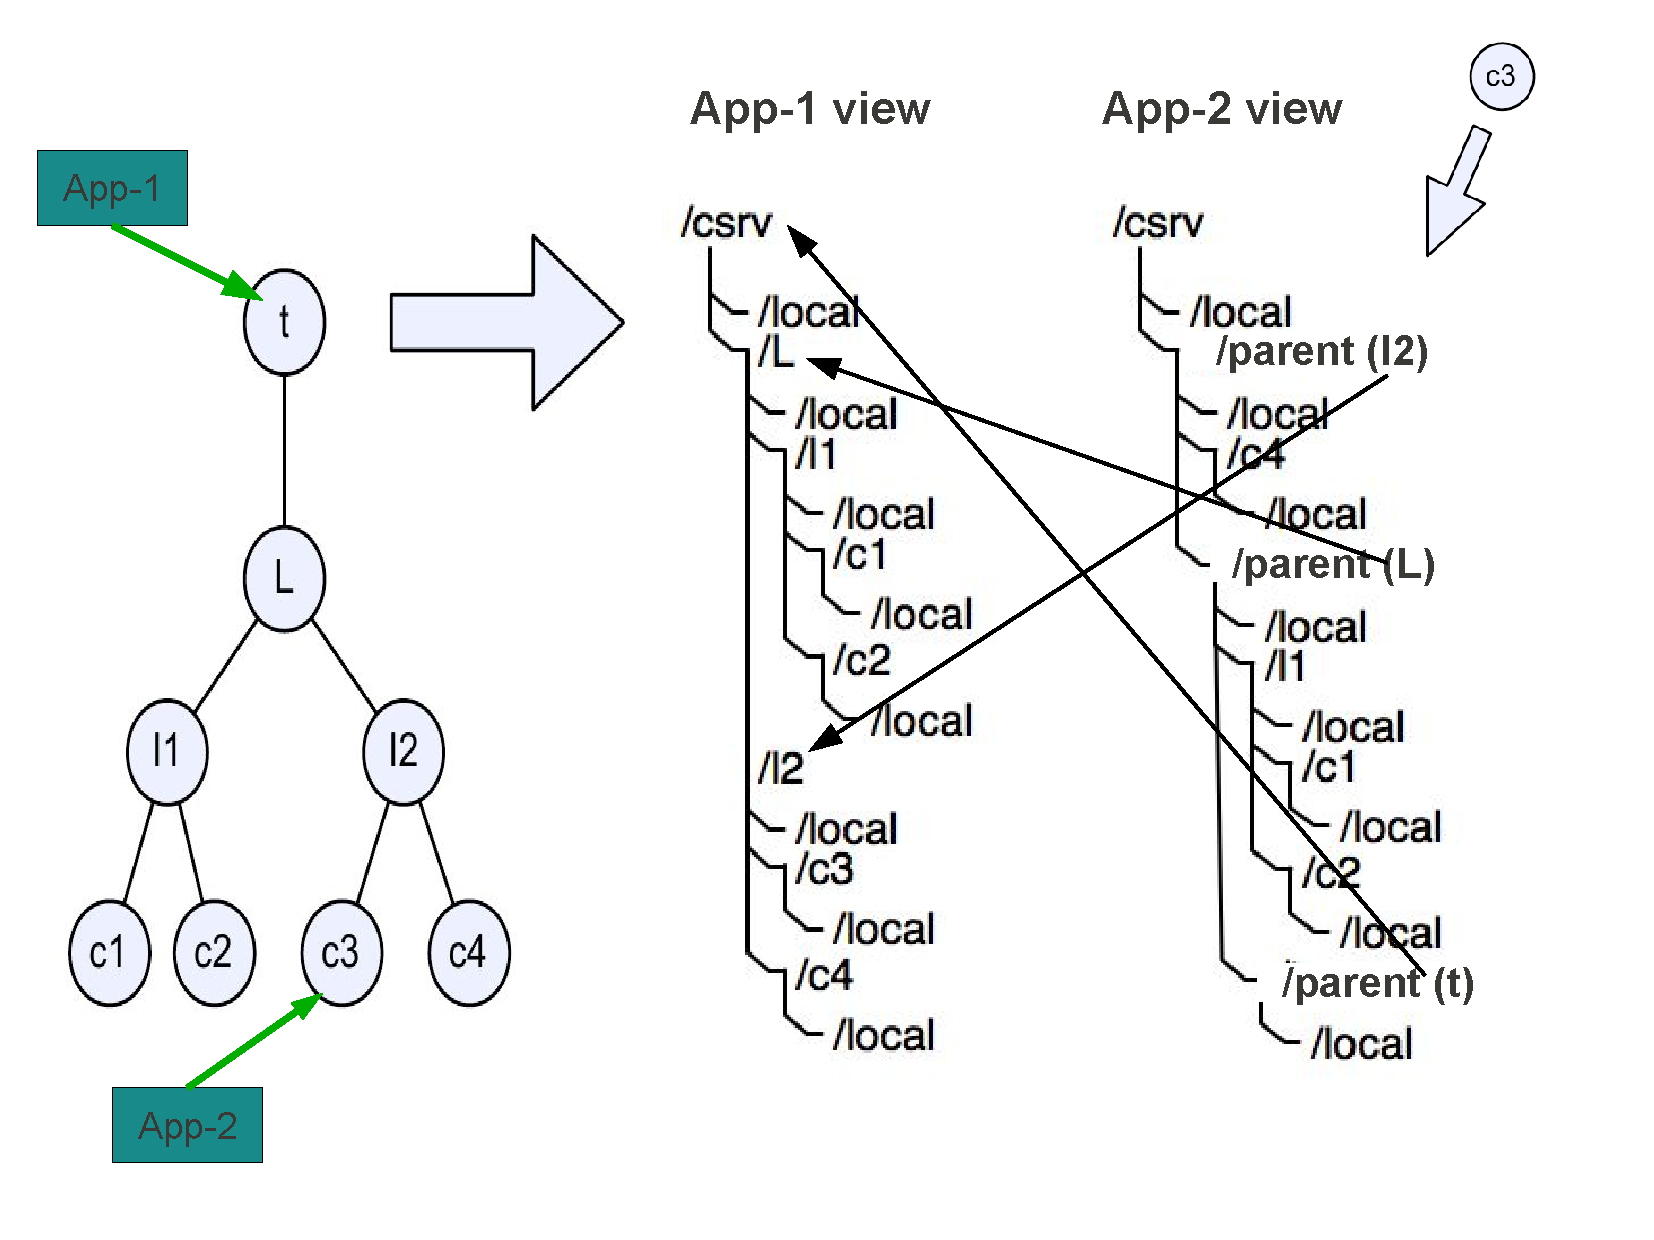
\includegraphics[height=0.3\textheight,width=0.4\textwidth]
		{./img/xcpu3FSTopo}
    \caption{Sample filesystem interface for sample the topology in XCPU3}
    \label{fig:xcpu3FSTopo}
  \end{center}
\end{figure}

Assuming the links between the nodes are created by the remote node mounts in
central services, this diagram shows how the filesystem views at different
nodes encompases the whole network, even though each node is only connected to
its neighbours. The XCPU3 filesystem starts with the \texttt{[/csrv]}
directory. The location \texttt{[/csrv/local/]} presents the local resources
whereas \texttt{[/csrv/parent/]} presents the XCPU3 filesystem of the parent
node. All other directories in the represents the XCPU3 filesystem of the
children nodes.  It can be easily seen that both \textit{App-1} and
\textit{App-2} have access to all the nodes even though they are running on
different nodes.  In this design, every node has to worry about only its
children and the parent, other topology falls in the place automatically.

Even though the filesystem view at different nodes differ from each other, 
all nodes have access to the full topology.  The \texttt{[/csrv/]} filesystem
view encodes enough information within itself that any nodes can construct the
global view and figure out their own position within the global view.

Just because every node can construct the global view, does not mean that it
must use this global view for making any decision or performing a typical
operation. The nodes mostly use only the local view for decision making and
operations. This local view includes the parent node and the children nodes.


\section{Filesystem Interface}

This section discusses the filesystem interface and how it can be used for
managing the local and remote resources. Figure \ref{fig:xcpu3Local} gives the
the high-level view of the hierarchy of the XCPU3 filesystem.  This section
will discuss the overall hierarchy and few important files in the XCPU3.

\begin{figure}[h]
  \begin{center}
    \leavevmode
      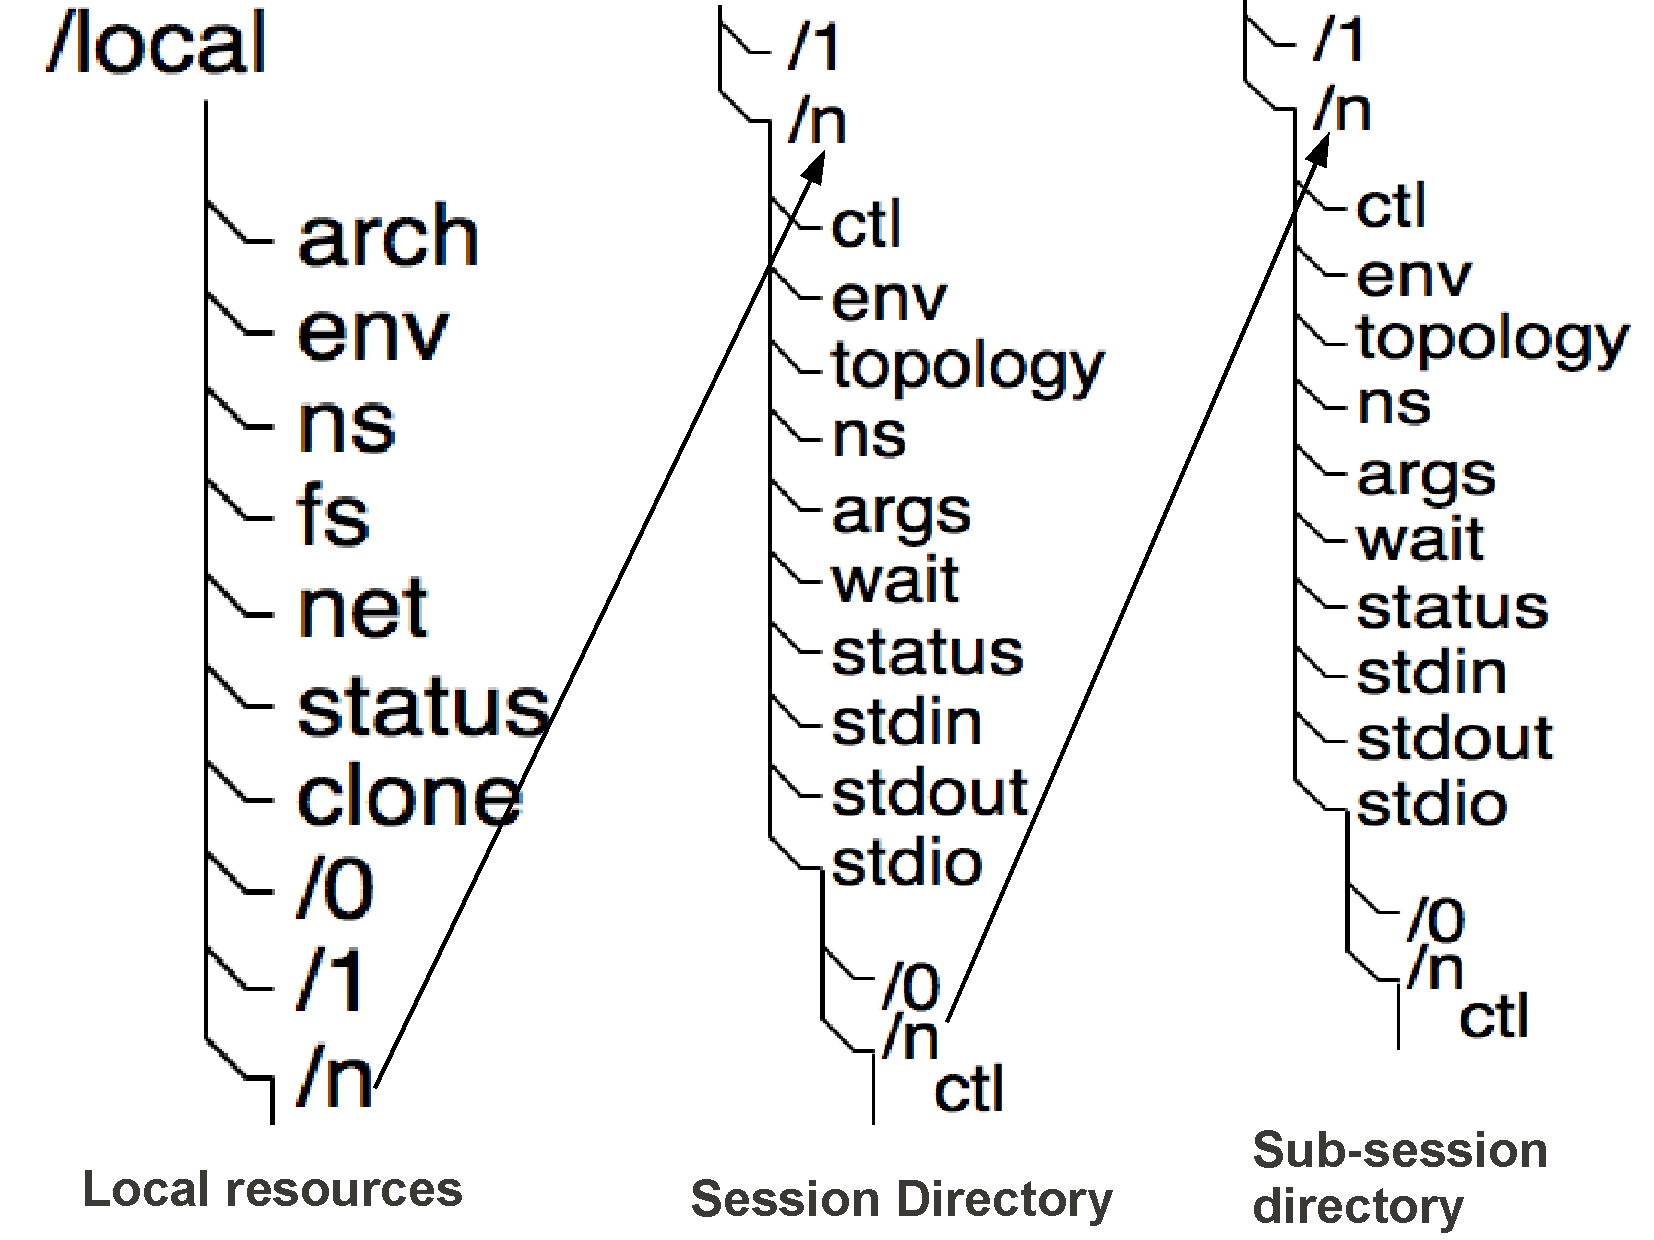
\includegraphics[height=0.25\textheight,width=0.4\textwidth]
		{./img/local_session_subsessions}
    \caption{Filesystem interface in XCPU3}
    \label{fig:xcpu3Local}
  \end{center}
\end{figure}

The location \texttt{[/csrv/local/]} points to the local resources available on
the node and the files present in this directory allows managing these local
resource. Few files here provide information about the system, like
\texttt{[arch]} file tells the architecture and operating system of the node
while \texttt{[status]} file provides information about total amount of
resources available, including the remote resources which are direct or
indirect decendents of this node.  Files like \texttt{[env]} and \texttt{[ns]}
allowed controlling the default environment and the namespace of the processes
created on this node.  \texttt{[fs]} and \texttt{[net]} are links to the local
filesystem and networking resources available on the node.  The
\texttt{[clone]} file provides the interface to create new sessions which is
the unit of the execution.

The sessions are represented as directories with session-id number as a name. 
These sessions are self-contained and provide interfaces to manage the
execution of the session.  Files like \texttt{[env]} and \texttt{[ns]} are
present is session directory also, and can be used to overwrite the default
environment and namespace specifically for this session.  File \texttt{[ctl]} is
used for controlling the execution and file \texttt{[stdio]} is used to
manipulate standard input and output.  Sessions can play one of the two roles
between \textit{single execution unit} and \textit{aggregation} of other
sessions. Following is the attempt to define these two modes.
\begin{verbatim}
SESSION -> AGGREGATION | execution
AGGREGATION -> SESSION+
\end{verbatim}
The \textbf{execution mode} executes the requested program and provides the
output.  The \textbf{aggregation} mode aggregates and manages the multiple
sessions which are created as sub-sessions for this session.  In other words,
aggregation session creates sub-sessions, divide the work among them and
aggregate back the output.  These sub-sessions are nothing but sessions created
by using \texttt{[clone]} file on local or remote systems.  These newly created
sessions are binded as sub-directories inside the current session directory.

\subsection{Workload distribution and aggregation}
The workload distribution and aggregation works by using the dual nature of
the sessions.  The first step in this is reservation, which is responsible for
creating the tree of the sessions.  Whenver any session receives the reservation
request, it evaluates it by considering, if it can execute locally or it should
break it and divide between its available children.  Depending on the decision,
it can play one of the following two roles.
\begin{enumerate}
  \item \textbf{Execution session}: When reservation is request is small enough
  or there are no children nodes available, then session behave as execution
  session by performing the requested operations locally.  The execution
  sessions are the leaf node in the session tree.
  
  \item \textbf{Aggregation session}: When request is bigger than what session
  can handle, it divides the request between children nodes.  The session does
  this by creating new session and sending the divided
  reservation request to the each child node available in it's \textbf{CSRV}
  hierarchy.  These newly created sessions will be binded as directories in the
  directory of the current session hance making them the sub-sessions of the
  current session.  The current session now acts as in aggregation point for
  these sub-sessions by passing the any execution request or input to all
  sub-sessions and merging the output from all sub-sessions to produce the final
  output.  These aggregation sessions constitute the non-leaf nodes in the
  session tree.
\end{enumerate}
This way, recursive tree of sessions is created whenever new reservation request
is received.  This tree of the session is then used to request the execution and
collect back the results.  This design not only distributes the actual
execution, but also it distributes the distribution and aggregation process as
this work is divided between all aggregation sessions.

\subsection{Examples}
It is hard to measure the \textit{ease of use} and \textit{simplicity}
factor.  So, we are presenting following examples to show how easy it is
to use XCPU3 infrastructure.  We are giving these examples of using the bash
shell in Linux.

\subsubsection{Traditional application deployment}
This example presents how the default aggregation behaviour of the XCPU3 can
used to deploy large number of applications.

We assume that the XCPU3 filesystem is mounted on \texttt{./mpoint/} directory. 
This can be done by using FUSE or 9VFS\cite{v9fseric}.
\begin{verbatim}
$ less ./mpoint/csrv/local/clone
0 
\end{verbatim}
The above command is an example of creating a new session. The contents read
from the \texttt{[clone]} file represent the session-ID.  Now we use session 0
for performing actual execution.
\begin{verbatim}
$ echo "res 4" > ./mpoint/csrv/local/0/ctl
$ echo "exec date" > ./mpoint/csrv/local/0/ctl
$ cat > ./mpoint/csrv/local/0/stdio
Fri May 7 13:53:58 CDT 2010
Fri May 7 13:53:58 CDT 2010
Fri May 7 13:53:58 CDT 2010
Fri May 7 13:53:58 CDT 2010
$
\end{verbatim}
The first echo command sends the request for reserving 4 remote resources. The
next echo command submits the request for executing the \texttt{date} command.
And the \texttt{cat} command on \texttt{[stdio]} returns the aggregated output
to the user.  This example shows all the complexities about finding, connecting
and using the remote resources is hidden behind the filesystem interface.
This approach can be used in the \textit{trivially parallelizable applications}
where the same application is deployed on all the nodes.

\subsubsection{Dataflow deployment}
In this mode the role of XCPU3 is limited to the reservation. An application
is given the capability of doing the workload distribution and aggregation
with the help of the filesystem interfaces provided by the XCPU3. Instead of
interacting with the aggregation points, these dataflow applications can
interact directly with the sessions responsible for the actual execution using
the filesystem hierarchy of that session.

In this example, we will try to create a small pipeline of two commands
\texttt{date | wc}.  But we will create this pipeline across multiple nodes. 
The objective of this example is to show how the underlying complexities are
hidden from the application.

Lets assume that session 0 is created by opening \texttt{[clone]} file as shown
in the previous example.  The following commands will create the desired
pipeline.

\begin{verbatim}
$ echo "res 2" > ./mpoint/csrv/local/0/ctl
$ echo "exec date" > ./mpoint/csrv/local/0/0/ctl
$ echo "exec wc" > ./mpoint/csrv/local/0/1/ctl
$ echo "xsplice 0 1" > ./mpoint/csrv/local/0/ctl
$ cat ./mpoint/csrv/local/0/1/stdio
1 6 29
$
\end{verbatim}

The first command \texttt{[exec date]} is sent to 0'th sub-session and the
second command \texttt{[exec wc]} is sent to the 1st sub-session.  The
\texttt{[xsplice 0 1]} request tells the parent session to redirect the output
of the 0'th session to the input of the 1st session.  The \textbf{xsplice}
command can be seen as a pipe operator of the shell script for redirecting the
output of one command to the input of other command.

The above example is equivalent of executing \texttt{date | wc} on the shell,
but with the difference that both commands are executed on a different remote
machines while sharing the same namespace.

The XCPU3 infrastructure relies on userspace applications like the \textbf{PUSH
shell}\cite{PODC:Push} for creating more complicated DAG and mapping them on
underlying XCPU3 infrastructure.

\section{Evaluation}

This section presents the evaluation of the XCPU3 infrastructure from the
perspective of quicker deployment of a large number of small jobs while giving
clean interfaces and abstractions.


\subsection{Experimental setup}
We have performed our evaluations on a Blue Gene setup with 512 nodes.  This
setup is visually presented in a figure \ref{fig:hare}.  We run hosted Inferno
on all the compute nodes, IO nodes and the controller node.  The user interacts 
with the XCPU3 instance on the controller node for job submission.


\begin{figure}[h]
  \begin{center}
    \leavevmode
      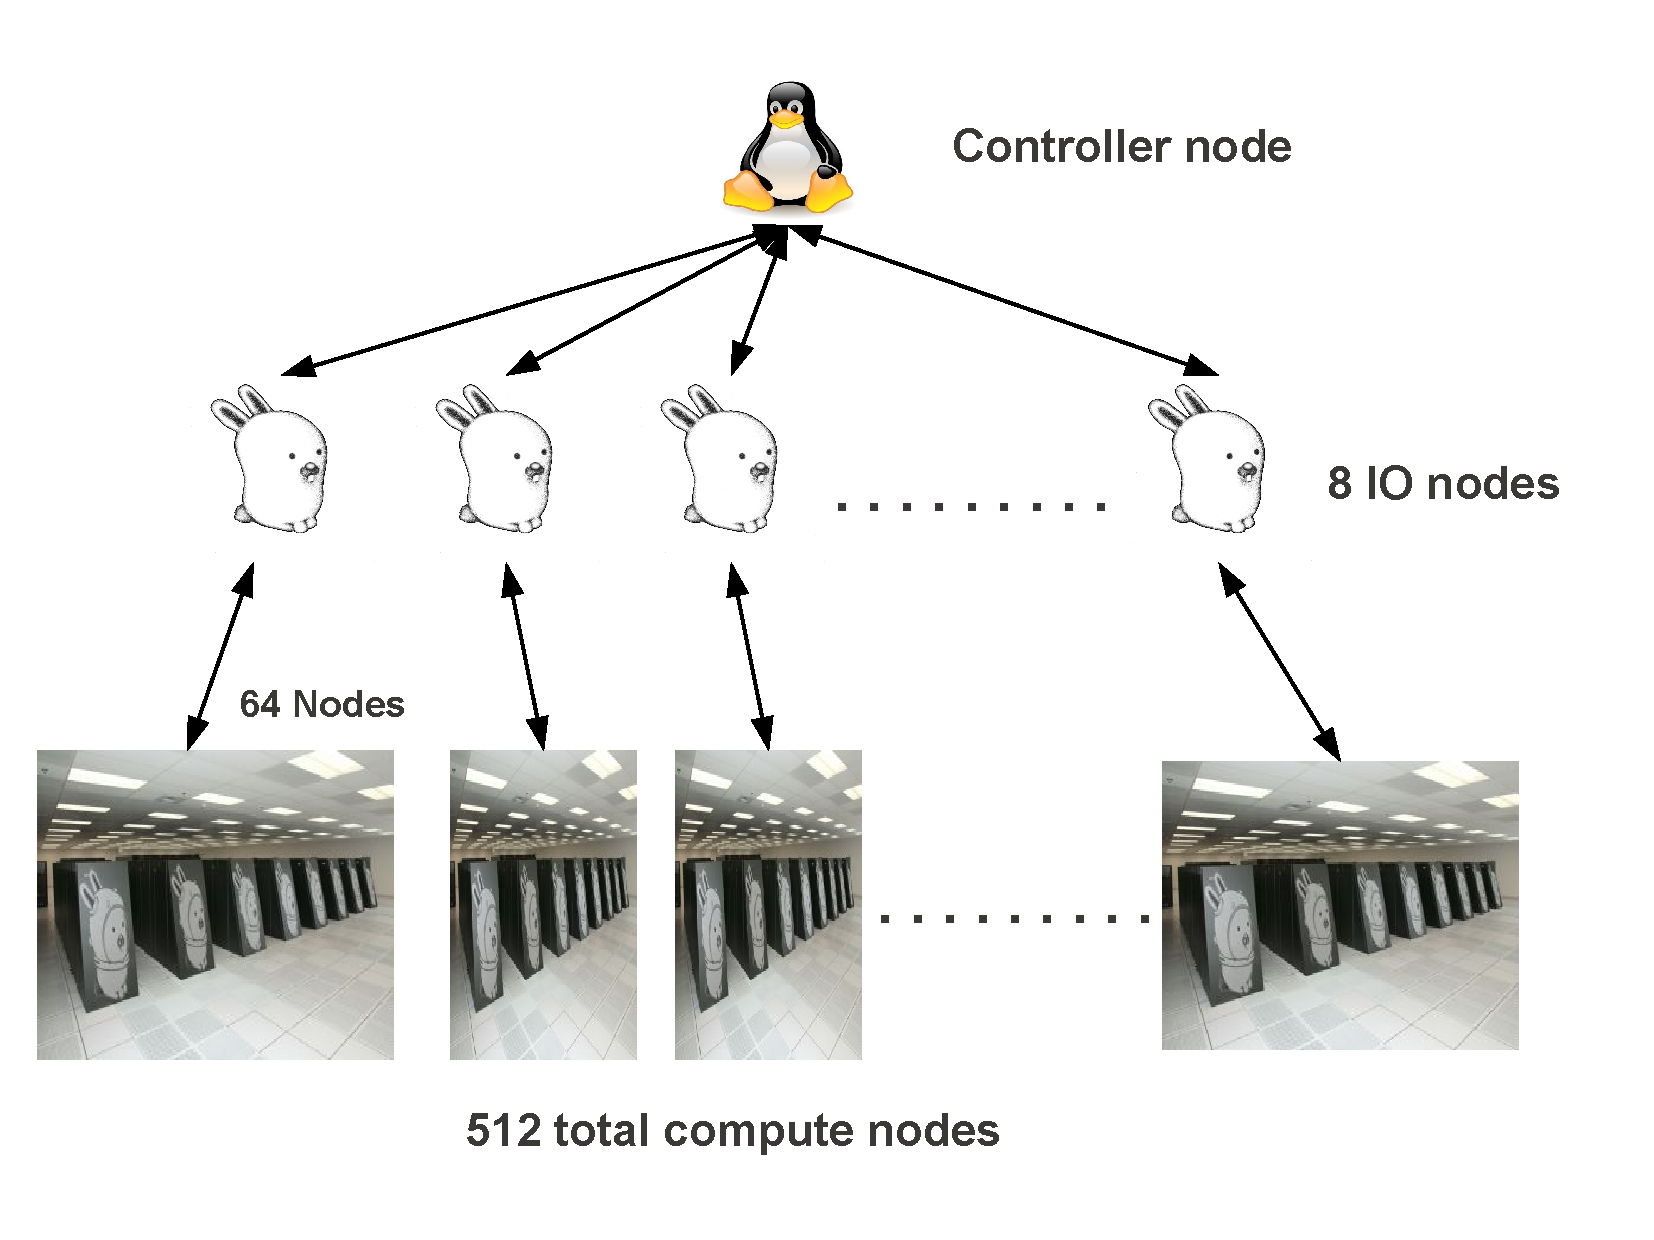
\includegraphics[height=0.2\textheight,width=0.4\textwidth]
		{./img/EvaluationSetup}
    \caption{Setup for evaluation}
    \label{fig:hare}
  \end{center}
\end{figure}


\subsubsection{Scalability of XCPU3}
Our first objective is to show how quickly we can do deployment and execution
of a large number of small applications. We have avoided using larger
applications as the bigger runtimes of larger applications tend to amortize the
overhead in the deployment of the application.  We have used the \texttt{date}
command as the application for deployment.  This is a small application and does
not need any external inputs and produces small output. Each deployment involves
session creation, reservation, execution, output aggregation and termination
of the session.  We deployed varying numbers of execution of this application on
the cluster of 512 nodes.  The number of requested executions increased
exponentially from 1 to 2048 executions.

\begin{figure}[h]
  \begin{center}
    \leavevmode
      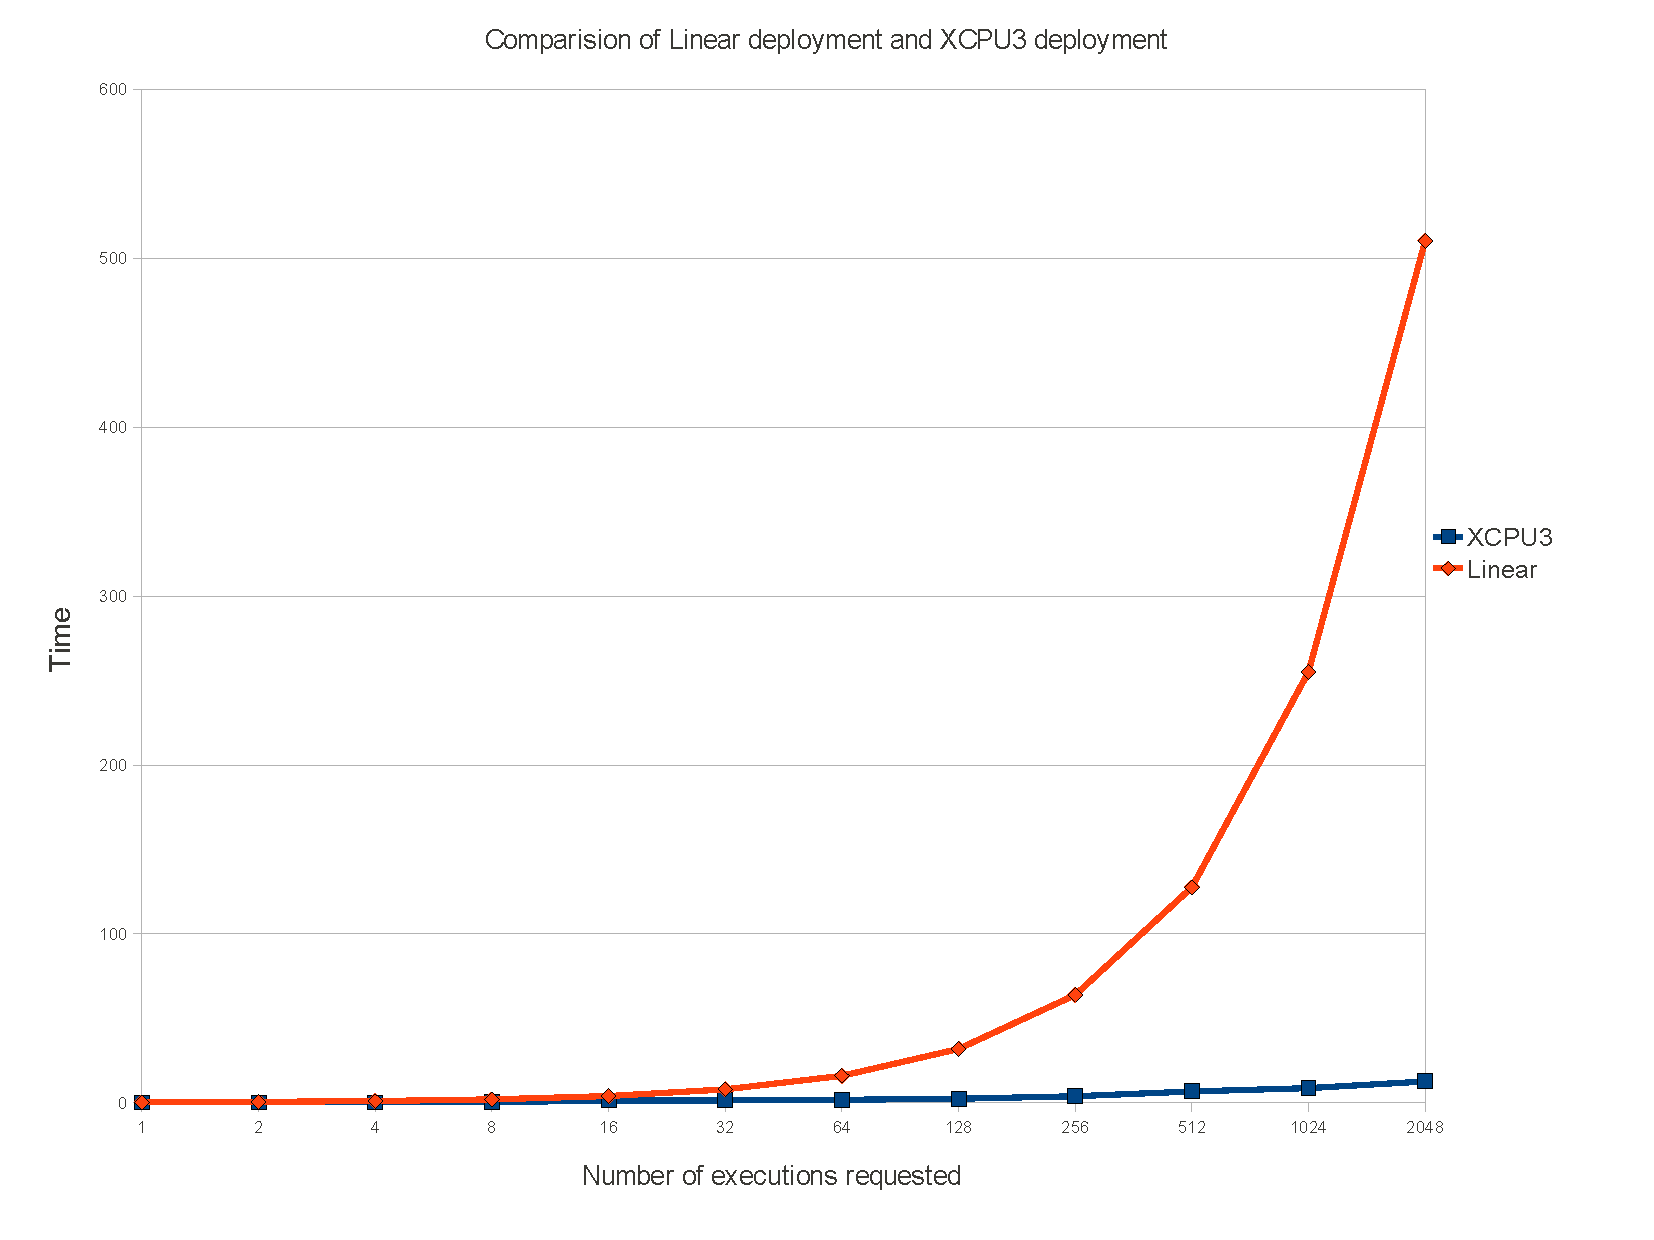
\includegraphics[height=0.2\textheight,width=0.5\textwidth]
		{./img/linear}
    \caption{Comparison if XCPU3 with sequential deployment}
    \label{fig:sequential}
  \end{center}
\end{figure}

Figure \ref{fig:sequential} gives an initial perspective of how XCPU3 performs
relative to sequential performance.  This graph plots the total time taken by
XCPU3 and the hypothetical time it may take for performing the same amount of
work on one machine.  This graph shows that the XCPU3 is successfully able to
exploit the parallelism for deploying the jobs quickly. The XCPU3 deploys 2048
jobs in 12.66 seconds whereas sequential execution would take upto 510 seconds.
In the graph, the line showing sequential scaling looks exponential, but that is
because number of requested executions increase exponentially.


\subsubsection{Job deployment without input}
This section aims to further analyze the performance of XCPU3.  Again we are 
concentrating on similar deployment.  We have recorded the time taken by each
of the following stages in the deployment on the XCPU3 infrastructure.

\begin{enumerate}
\item Reservation: Create a new session, and request the reservation by writing
\texttt{res n} into the session \texttt{[ctl]} file.  Here \textbf{n} varies
from 1 to 2048 representing the number of executions requested. 

\item Execution: Request the execution by writing \texttt{exec date} into the
session \texttt{[ctl]} file.

\item Aggregation: Collect the output generated by all the executions by reading
the session \texttt{[stdio]} file.

\item Termination: Closing all the files and terminating the session.

\item Housekeeping: Additional time taken before, between and after above steps.
\end{enumerate}
Every deployment starts with the creation of the session followed by the
reservation, execution, aggregation and then ending with termination of the
session.  We have taken the average value over multiple runs for our analysis.

\begin{figure}[h]
  \begin{center}
    \leavevmode
      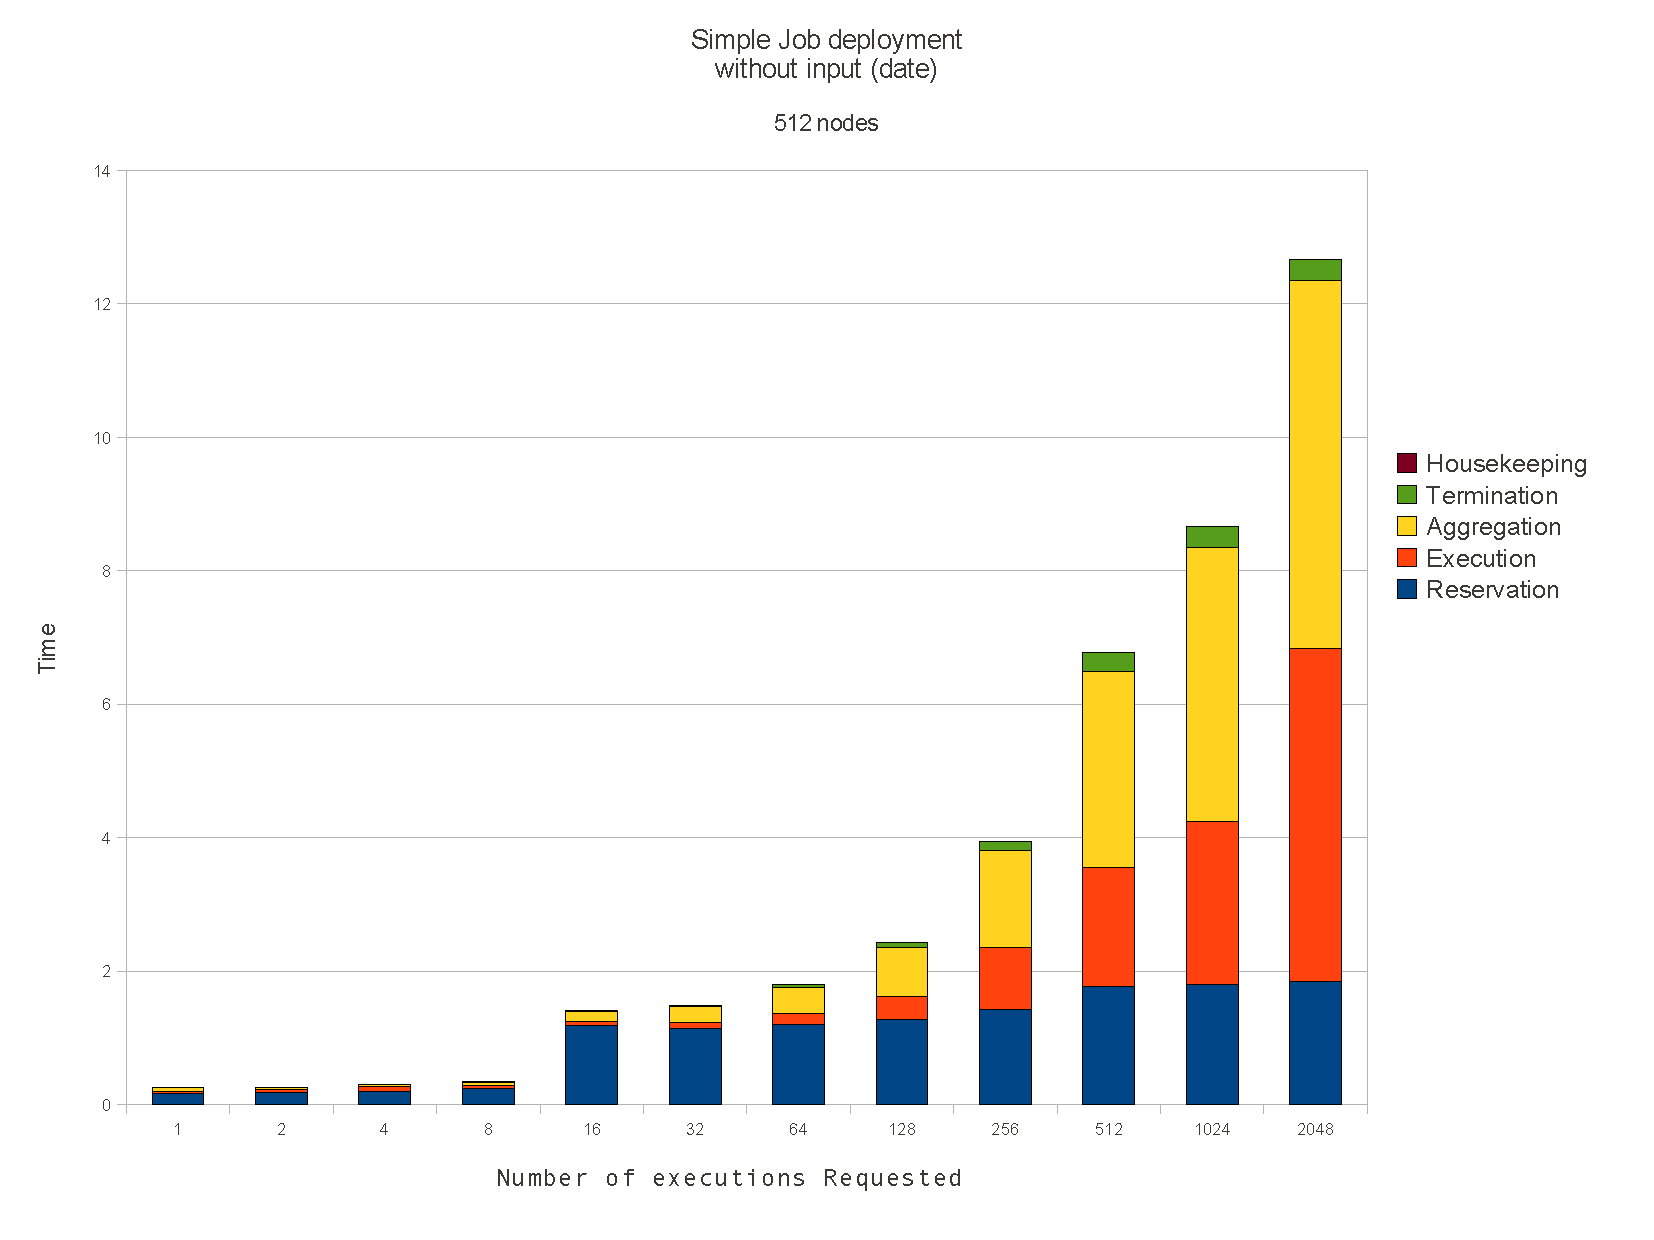
\includegraphics[height=0.2\textheight,width=0.5\textwidth]
		{./img/date_graph}
    \caption{Deployment without input}
    \label{fig:date_graph}
  \end{center}
\end{figure}

Figure \ref{fig:date_graph} presents the results of deployment of the date
command in the form of graph.  This graph presents the breakup time for various
stages of the deployment using the XCPU3 infrastructure.

From this graph we can observe that the session termination and the housekeeping
overheads are negligible compared to the time taken by reservation, execution
and aggregation.  So, we can ignore these two overheads in our future
evaluations.  For jobs of up to 128 deployments, the reservation time dominates
everything else.  But for larger numbers of deployment execution and
aggregation time increases rapidly while reservation time remains relatively
constant. This shows that reservation time is not directly dependent on
the number of deployments, whereas execution and aggregation time are directly
proportional to the number of deployments.

Now, let us try to analyze why reservation time is independent of the number of
deployments.  The reservation process involves traversing the underlying
topology tree of nodes till the reservation requirements are satisfied.  All the
children on the same level are traversed parallelly at the same time.  This way,
each level is traversed in the constant time, independent of number of nodes in
that level.  Another aspect of the reservation mechanism which helps here is
that the amount of data written and read from the \texttt{[ctl]} file and the
amount of data exchanged between nodes for communicating reservation request is
fixed in size and independent of the number of deployments requested.  With
these two properties, the reservation time becomes directly proportional to the
depth of the tree and not with the number of nodes.

We can observe the above relation in figure \ref{fig:date_graph}. The 
reservation time remains relatively constant for deployment requests from 1 to
8.  Then it sharply increases between 8 to 16 and remains almost constant for
all the requests between 16 to 2048.  This can be attributed to underlying
cluster topology. Figure \ref{fig:hare} shows the presence of the 8 IO nodes
in the first level. This enables satisfying the requests which are smaller
than 8 executions. For larger requests, one more level needs to be traversed
in the topology, introducing delays.  The time taken for reservation remains
almost constant between 16 and 2048 executions as all these reservation
requests essentially traverses the same depth.  We can conclude from these
observations that \textit{the time taken for the reservation is directly
proportional to the depth of the tree}.


Now let us discuss, why the same property is not exhibited by execution time or
aggregation time. We have discussed in the implementation chapter that all
read and write requests are performed in parallel between all the nodes in the
same level.  But the amount of data exchanged for aggregation and execution is
not constant.  This data is directly proportional to the number of nodes
involved.  With the increase in the number of requested deployments, the
amount of data to be exchanged also increases, leading to larger aggregation
time. The execution time is also similarly affected as all compute nodes will
try to fetch the binary of the executable from the initiating node leading to
the copy of the data. These observations lead us to to conclusion that
\textit{the time taken for the execution and aggregation is directly
proportional to the number of deployments requested}.

\subsubsection{Job deployment with input}
Our next evaluation involve the deployment of an executable \texttt{wc} which
needs input. This command counts the number of lines, words and characters in
the input file.  This is an interesting case for our infrastructure as this
deployment involves the distribution of inputs to all the sessions.  This
introduces a new stage in the deployment process in addition to the 5 stages we
described in the above section.  This stage will be the \textbf{input} stage and
involves distributing the input data to all the sessions which are responsible
for execution.  By default XCPU3 will broadcast the input to all the compute
nodes, but we have plans to introduce filters in the PUSH shell which can
partition the input given to the compute  nodes. 

Figure \ref{fig:wc_graph} presents the results of evaluations involving the
distribution of the input.


\begin{figure}[h]
  \begin{center}
    \leavevmode
      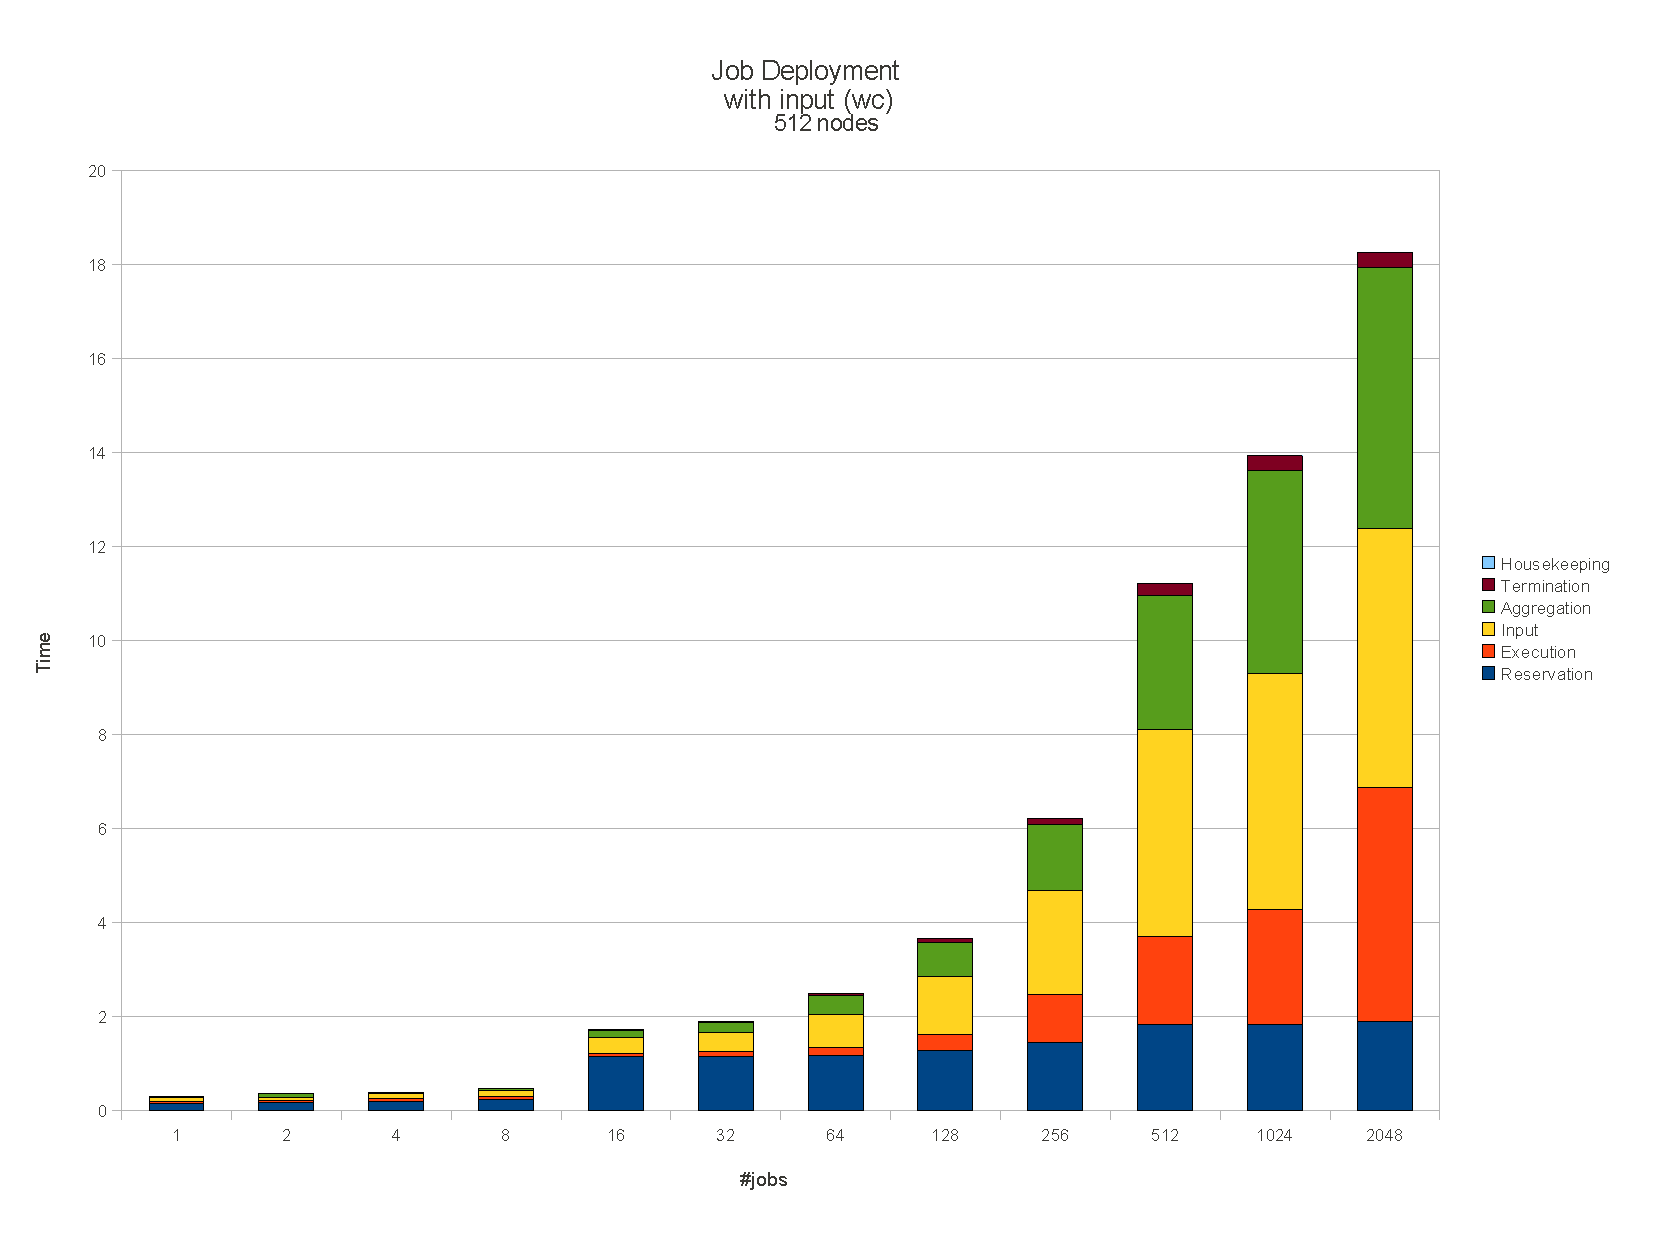
\includegraphics[height=0.2\textheight,width=0.5\textwidth]
		{./img/wc_graph}
    \caption{Deployment with input}
    \label{fig:wc_graph}
  \end{center}
\end{figure}

These results enforce our observations that reservation time is directly
proportional to the the depth of the tree whereas aggregation and execution time
are directly proportional to the number of deployments requested.  In addition
to these observations, we can also observe that the input time exhibits 
behavior similar to the execution and aggregation time.  This observation can be
attributed to the fact that input distribution implementation is similar
to the output aggregation implementation.  And also the amount of data to be
exchanged for input distribution depend on the number of deployments requested
as this data needs to reach all sessions responsible for execution.  This
increases the amount of data to be exchanged with any increase in the number of
the deployments requested.  We can conclude with this observation that
\textit{the input time is directly proportional to the number of deployments
requested}


\subsection{Dataflow workloads}
The evaluations presented in this chapter helps us in understanding how fast
XCPU3 can deploy small jobs and aggregate the results produced by them.  Now
let us relate how these observations can justify our claims about dataflow
applications. Typical deployments of the dataflow applications are similar to
the above experiments as it involves starting up a large number of small jobs.
But the similarity is over at this point. Dataflow deployment does not always
involve the input distribution and output aggregation stages.  These deployments
work by feeding the output of one computation as input for other computation. 
At the end of the computation, a user needs to read the output of only selected
compute sessions which does not need any aggregation.  What we can conclude from
the above description is that XCPU3 performs really well in the stages like
reservation which are important for dataflow deployments.  The stages like input
distributions are output aggregation where XCPU3 is relatively slow are not
needed by dataflow deployments.  This makes XCPU3 ideal for rapid deployment of
dataflow workloads.

Unfortunately we do not have concrete measurements and evaluations to back our
predictions.  XCPU3 is one of the piece in the envisioned solution for problem
of efficient and easy deployment of large-scale dataflow applications.   We are
still working on the integration of userspace applications like
PUSH\cite{PODC:Push} with XCPU3 which will further simplify the dataflow
deployment.


XCPU3 is an infrastructure which provides the needed flexibility, speed and 
ease of use for dataflow workloads.  This chapter demonstrates the speed that
can be achieved.  It is difficult to measure the properties like \textit{ease of
use} and \textit{flexibility} but the examples presented in the filesystem
interface chapter should give some insights of all the possibilities opened up
by the XCPU3.


\section{Related work}


This section tries to put XCPU3 in the context of other work which 
has been done in this area.  We will briefly discuss the various related
projects and how they differ from XCPU3.

\subsection{Historical solutions}
The concept of workload distribution between multiple machines was introduced in
the research by research projects like Amoeba \cite{amoeba} and Cambridge
distributed computing system\cite{Needham82}.  These were developed as a general
purpose distributed operating system which can solve the problem of scarcity
of compute resources. These systems introduced many useful concepts, but easy
availability of PC made these systems outdated.

\subsection{Traditional solutions}
As we are approaching the limits on silicon technologies the trend has changed
to design of multicore and manycore chips and increased the use of clusters and
grids. These clusters and grids had independent operating system on each
machine and were loosely coupled using networking.  This lead to the
remote process management based on remote login and remote shells like
SSH\cite{ssh}.  Most of the existing middleware and workload distribution
systems use the above approach with wrappers to simplify the user interface.

The limitation of using SSH is that the application has to run in the
namespace of the compute node instead of client node. And as SSH connections
are one-to-one, they do not scale well for managing large number of remote
nodes.  Attempts like Parallel SSH (PSSH)\cite{pssh} to overcome this
limitation of scalability but at cost of losing the flexibility of fine grained
control.

\subsection{BProc}
\textit{BProc: Beowulf Distributed Process Space} \cite{bproc} is developed as
an alternative to the loosely coupled SSH based job deployment. BProc works by
tightly coupling the kernels running on cluster nodes and provides distributed
process ID space which allows a front node to locally control all remotely
started processes.

Bproc is definately a step towards more control on remote processes but needs
modified kernel on all systems and remote processes still run in remote
namespace instead of the client namespace. These restrictions lead to the
loses of the flexibility which is needed for dynamic workloads.

\subsection{Multicast Reduction Network (MRNet)}
The MRNet\cite{MRNet} is designed for efficient multicast and data aggregation.
This project concentrates on optimizing group communication but it is language
dependent.  The MRNet API is in C++ and one needs to develop the applications
using this API leading to lot more efforts from the developer side to use this
infrastructure in comparison to XCPU3.

\subsection{Streamline}
The idea of using filesystem interface for data-streams is also used by the
\textit{pipefs}\cite{1400104} which is part of the streamline\cite{streamline}
project.  This approach of using filesystem interface is quite similar to
XCPU3, but the objectives of both these projects are different. Pipefs
concentrates on faster I/O with filesystem interface for the Linux kernel
while XCPU3 concentrate on the flexible workload management.


\subsection{Dryad}
Dryad\cite{yu2008dsg} is a distributed engine for data-parallel applications
which is designed with a primary focus on simplicity of the programming model,
reliability, efficiency and scalability.  Dryad is well suited for dataflow
applications where amount of computation needed is already known.  But it does
not provide way to dynamically adjust the reservations to deal with changing
workloads.    

Dryad addresses the issues like fault tolerance which are currently ignored by
XCPU3, but XCPU3 is more flexible as it can support dynamic workload and
changing DAG of dataflow deployments. Also the filesystem interface of the XCPU3
is much simpler and cleaner compared to the class based C++ interface of Dryad.

\subsection{Condor}
Condor\cite{condor-practice} is \textit{high-throughput distributed batch
computing} system which exploits \textit{opportunistic computing} and idle CPU
cycles of voluntary workstations for better performance.  Condor works by
breaking the large problem into smaller tasks and submitting these smaller
tasks to voluntary workstations. Condor handles scientific workflow
application by using the meta-scheduler DAGMan (Directed Acyclic Graph Manager)
which allows user to specify the various dependencies within tasks in form of
directed acyclic graph. 

Unfortunately, the volutary model for condor restricts the direct commnication
between the workstations for security reasons.  They typically communicate
only with the agent responsible for submitting the job.  This lack of the
ability to communicate directly with other computational nodes limit the
usefulness of Condor for communication intensive dataflow applications.

\subsection{Other commercial solutions}
There are few commercial Workload deployment solutions available.  The
\textit{Oracle Grid Engine}\cite{oge} is a batch-queuing system which can
accept, schedule, dispatch and manage the remote executions on clusters. 
Other solutions involve \textit{PBS Works}\cite{pbsworks} which is workload
and resource management solution and \textit{platform LSF (Load Sharing
Facility)}\cite{platformLSF} batch job scheduler which is aimed to help in
scheduling jobs on private clouds.  Most of these solutions target to simplify
the resource management and job submission/scheduling, but they do not try to
simplify the communication issues within applications.

\section{Future work}
The XCPU3 is an infrastructure which we plan to extend it further to support
fault tolerance and add capability to selectively restarting the sub-sessions
for environment where faults are more frequent.

As XCPU3 is filesystem interface and can be implemented by any filesystem, we
plan to implement this interface natively on traditional operating systems to
improve the performance by avoiding the virtualization layer added by the
Inferno.

\section{Conclusion}
XCPU3 project was initiated with the goal of creating alternate job deployment
mechanism primarily for menytask and dataflow deployments which can deal with
dynamic workloads. We have kept the design simple with the assumption that
simple design leads to the better scalability and flexibility.  We have tried
to show that from examples that the XCPU3 interfaces are easy to use in
language and runtime independent fasion. And with evaluation section we have
tried to prove that the XCPU3 is viable option for scalable deployment of
many-task and dataflow workloads.


\bibliography{references}

\end{document}
